\chapter{Magnétisme}
\section{Introduction}
Les phénomènes magnétiques sont connus en Europe depuis l'Antiquité grecque peut-être même depuis l'époque sumérienne (4000 ans av. J.-C.). Le premier à qui l'on attribue véritablement la découverte de l'aimantation, c'est le philosophe grec Platon (427 av. J.-C. -- -347 av. J.-C.). L'observation du magnétisme repose sur la découverte de pierres qui pouvaient attirer le fer. Ces pierres ont été découvertes dans la région de Magnésie en Asie mineure, cette région a donc donné le nom de magnétisme au phénomène.

La boussole fait son apparition en Europe vers la fin du \textsc{xii}\ieme~siècle. Pour les Chinois, cette découverte remonte à une époque plus ancienne: le médecin Shen Gua (1031--1095) décrivait déjà une aiguille indiquant le sud lorsqu'elle était frottée par la pierre d'aimant.
\textbf{Le magnétisme correspond aux effets exercés par les charges en mouvement sur d'autres charges en mouvement.}

\newpage

\begin{tcolorbox}[colback=mygray1,breakable,colframe=mygray2,sharp corners=northwest,title={Magnétisme animal, Mesmer et pseudo-sciences}]
    Pour certaines personnes, la première chose qu'évoque le mot magnétisme est la pratique des \enquote{magnétiseurs}, étroitement liée à celle des sourciers, des pendules et des \enquote{guérisseurs} non scientifiques.
    Cette confusion date en grande partie du \textsc{xviii}\ieme~siècle, lorsque Franz-Anton Mesmer développe l'idée d'un magnétisme animal pouvant être généré par certaines personnes et pouvant avoir une influence sur les autres. Louis \textsc{xvi} ordonne en 1784 deux commissions --- auxquelles participeront Antoine Lavoisier et Benjamin Franklin --- pour enquêter sur ces étranges séances magnétiques. Les enquêteurs concluent à l'absence de fondements du magnétisme animal.

    Plus récemment, de nombreuses études scientifiques ont démontrées que les sourciers ne détectent pas mieux les sources d'eau que ne le ferait le simple hasard. Pourtant, les charlatans, le plus souvent de bonne foi, prospèrent et utilisent le vocabulaire scientifique (champ, magnétisme, fluide, force, \ldots) pour donner l'illusion que leurs pratiques auraient un fondement rationnel.
\end{tcolorbox}

\newpage

\section{Les aimants permanents}
Les aimants attirent les clous, les trombones ou tout autre objet en fer mais aussi le cobalt, nickel et certains alliages. Quelle que soit sa forme, allongée ou en U, il comporte toujours deux extrémités appelées \motcle{pôles}, où les effets magnétiques qu'il produit sont le plus marqué. Lorsqu'un aimant peut s'orienter librement, un de ses pôles, appelé par convention le pôle nord de l'aimant, s'oriente vers le pôle Nord géographique de la Terre. C'est le principe de la boussole.
\begin{figure}[h!]
    \centering
    {\begin{tikzpicture}
\tikzset{>=latex}
\tkzInit[xmin=-5,xmax=5,ymin=-5,ymax=5]
\tkzClip
\begin{scope}[rotate=11]
\tkzDefPoint(0,2){A}
\tkzDefPoint(0,-2){B}
\tkzDefPoint(0,0){O}
\tkzDrawCircle[fill=mygray1](O,A)
\tkzDefPointBy[rotation=center O angle -11](A)
\tkzGetPoint{Ngeog}
\tkzDefPointBy[rotation=center O angle -11](B)
\tkzGetPoint{Sgeog}

%1_droite
\draw (.9,0) [ 
color=NavyBlue,
decoration={markings, mark=at position 0 with {\arrow{>}}},
postaction={decorate}] 
ellipse (.9  and .6);

%1_gauche
\draw (-.9,0)[
color=NavyBlue,
decoration={markings, mark=at position 0.5 with {\arrow{<}}},
postaction={decorate}] 
 ellipse (.9  and .6);

%2_droite
\draw (1.5,0) [
color=NavyBlue,
decoration={markings, mark=at position 0.125 with {\arrow{>}}},
postaction={decorate}]
ellipse (1.5  and 1);%rapport=0.67

%2_gauche
\draw (-1.5,0) [
color=NavyBlue,
decoration={markings, mark=at position 0.375 with {\arrow{<}}},
postaction={decorate}]
 ellipse (1.5  and 1);

%3_droite
\draw (2,0) [
color=NavyBlue,
decoration={markings, mark=at position 0.25 with {\arrow{>}}},
postaction={decorate}]
 ellipse (2  and 1.5);%rapport=0.75

%3_gauche
\draw (-2,0) [
color=NavyBlue,
decoration={markings, mark=at position 0.25 with {\arrow{<}}},
postaction={decorate}]
 ellipse (2  and 1.5);

%4_droite
\draw (2.5,0) [
color=NavyBlue,
decoration={markings, mark=at position 0.375 with {\arrow{>}}},
postaction={decorate}]
ellipse (2.5  and 2);%rapport=0.8

 %4_gauche
\draw (-2.5,0) [
color=NavyBlue,
decoration={markings, mark=at position 0.125 with {\arrow{<}}},
postaction={decorate}]
 ellipse (2.5  and 2);

%5_droite
\draw (3,0) [
color=NavyBlue,
decoration={markings, mark=at position 0.375 with {\arrow{>}}},
postaction={decorate}]
 ellipse (3  and 2.55);%rapport=0.85

%5_gauche
\draw (-3,0) [
color=NavyBlue,
decoration={markings, mark=at position 0.125 with {\arrow{<}}},
postaction={decorate}]
 ellipse (3  and 2.55);

%6_droite
\draw (3.5,0) [
color=NavyBlue,
decoration={markings, mark=at position 0.375 with {\arrow{>}}},
postaction={decorate}]
 ellipse (3.5  and 3.15);%rapport=0.9

%6_gauche
\draw (-3.5,0) [
color=NavyBlue,
decoration={markings, mark=at position 0.125 with {\arrow{<}}},
postaction={decorate}]
 ellipse (3.5  and 3.15);

%7_droite
\draw (4,0) [
color=NavyBlue,
decoration={markings, mark=at position 0.375 with {\arrow{>}}},
postaction={decorate}]
ellipse (4  and 3.8);%rapport=0.95

%7_gauche
\draw (-4,0) [
color=NavyBlue,
decoration={markings, mark=at position 0.125 with {\arrow{<}}},
postaction={decorate}]
 ellipse (4  and 3.8);

%8_droite
\draw (4.5,0) [
color=NavyBlue,
decoration={markings, mark=at position 0.375 with {\arrow{>}}},
postaction={decorate}]
 ellipse (4.5  and 4.5);%rapport=1

%8_gauche
\draw (-4.5,0) [
color=NavyBlue,
decoration={markings, mark=at position 0.125 with {\arrow{<}}},
postaction={decorate}]
 ellipse (4.5  and 4.5);

\tkzDrawSegment[dashed,add=.1 and .1](A,B)
\tkzDrawSegment[dashed,add=.3 and .3](Sgeog,Ngeog)
\tkzLabelSegment[pos=1.2,right](Sgeog,Ngeog){\tiny Axe de rotation}



%\tkzMarkAngle[mark=none,size=0.5](Ngeog,O,A)
\tkzLabelAngle[pos=1.8](Ngeog,O,A){\tiny \(11^{\circ}\)}




\tkzDrawPoints(A,B,Ngeog,Sgeog)
\tkzLabelPoint[above left](A){\(S_{mag}\)}
\tkzLabelPoint[right](B){\(N_{mag}\)}
\tkzLabelPoint[right](Ngeog){\(N_{geog}\)}
\tkzLabelPoint[left](Sgeog){\(S_{geog}\)}





\draw [color=black,fill=Green,join=round] (-.1,0) rectangle (.1,0.5);
\draw [color=black,fill=BrickRed,join=round] (-.1,0) rectangle (.1,-0.5);
\draw (0,0.2) [color=black] node {\tiny S};
\draw (0,-0.2) [color=black] node {\tiny N};

\draw [color=black,fill=BrickRed,join=round] (2.9,0) -- (3,0.5) -- (3.1,0) -- cycle;
\draw [color=black,fill=Green,join=round] (2.9,0) -- (3,-0.5)-- (3.1,0)--cycle;
\draw (3,0.2) [color=black] node {\tiny N};
\draw (3,-0.2) [color=black] node {\tiny S};

\end{scope}
\end{tikzpicture}
}
    \caption{Pôles magnétiques et géographiques ; Nord et Sud.}
    \label{champ_magnetique_terre}
\end{figure}

\newpage
À l'instar des charges électriques, les pôles des aimants peuvent s'attirer ou se repousser. Deux pôles de même signe se repoussent, deux pôles de signes contraire s'attirent. Ceci implique qu'au Nord de la Terre se trouve un pôle sud magnétique\footnote{De nombreuse images disponibles sur Internet présentent de manière erronée un pôle magnétique nord au Nord de la Terre.}!


\begin{figure}[h!]
    \centering
    \resizebox{.7\linewidth}{!}
    {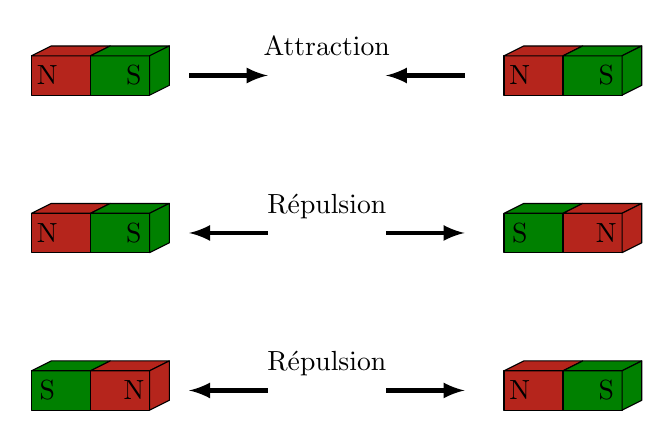
\begin{tikzpicture}
\tikzset{>=latex}

\newcommand{\unaimantNS}{
\draw [color=black,fill=BrickRed,join=round] (0,0) rectangle (.75,0.5);
\draw [color=black,fill=Green,join=round] (.75,0) rectangle (1.5,0.5);
\draw [color=black,fill=BrickRed,join=round] (0,0.5) -- (0.25,0.625) -- (1,0.625) -- (.75,0.5) --cycle;
\draw [color=black,fill=Green,join=round] (.75,0.5)-- (1,0.625) -- (1.75,0.625)--(1.5,0.5)--cycle;
\draw [color=black,fill=Green,join=round] (1.5,0.5) -- (1.75,0.625) -- (1.75,0.125) -- (1.5,0)--cycle;

\draw (0.2,0.25) [color=black] node {N};
\draw (1.3,0.25) [color=black] node {S};
}

\newcommand{\unaimantSN}{
\draw [color=black,fill=Green,join=round] (0,0) rectangle (.75,0.5);
\draw [color=black,fill=BrickRed,join=round] (.75,0) rectangle (1.5,0.5);
\draw [color=black,fill=Green,join=round] (0,0.5) -- (0.25,0.625) -- (1,0.625) -- (.75,0.5) --cycle;
\draw [color=black,fill=BrickRed,join=round] (.75,0.5)-- (1,0.625) -- (1.75,0.625)--(1.5,0.5)--cycle;
\draw [color=black,fill=BrickRed,join=round] (1.5,0.5) -- (1.75,0.625) -- (1.75,0.125) -- (1.5,0)--cycle;

\draw (0.2,0.25) [color=black] node {S};
\draw (1.3,0.25) [color=black] node {N};
}

\newcommand{\deuxaimantsNS}{
\unaimantNS

\begin{scope}[shift={(6,0)}]
\unaimantNS
\end{scope}
\draw[->,ultra thick](2,0.25)-- (3,0.25);
\draw[->,ultra thick](5.5,0.25)-- (4.5,0.25);
\draw (3.75,.5) [color=black,anchor=base] node {Attraction};
}

\newcommand{\deuxaimantsNN}{
\unaimantNS
\begin{scope}[shift={(6,0)}]
\unaimantSN
\end{scope}
\draw[<-,ultra thick](2,0.25)-- (3,0.25);
\draw[<-,ultra thick](5.5,0.25)-- (4.5,0.25);
\draw (3.75,.5) [color=black,anchor=base] node {Répulsion};
}

\newcommand{\deuxaimantsSS}{
\unaimantSN
\begin{scope}[shift={(6,0)}]
\unaimantNS
\end{scope}
\draw[<-,ultra thick](2,0.25)-- (3,0.25);
\draw[<-,ultra thick](5.5,0.25)-- (4.5,0.25);
\draw (3.75,.5) [color=black,anchor=base] node {Répulsion};
}

\deuxaimantsNS

\begin{scope}[shift={(0,-2)}]
\deuxaimantsNN
\end{scope}

\begin{scope}[shift={(0,-4)}]
\deuxaimantsSS
\end{scope}

\end{tikzpicture} 
 
}
    \caption{Attraction et répulsion entre les pôles des aimants.}
    \label{ar_aimants_droits}
\end{figure}

\newpage

\subsection{Monopôle magnétique}
\begin{wrapfigure}[10]{r}{0.3\textwidth}
    \vspace{-\baselineskip}
    \begin{tikzpicture}
\usetikzlibrary{decorations.pathmorphing}
\tikzset{>=latex}

\begin{scope}[shift={(-1.25,0)}]
\draw [color=black,fill=BrickRed,join=round] (0,0) rectangle (1.25,0.5);
\draw [color=black,fill=Green,join=round] (1.25,0) rectangle (2.5,0.5);

%les diagonales font ++0.25 en X ; ++0.125 en Y 

\draw [color=black,fill=BrickRed,join=round] (0,0.5) -- (0.25,0.625) -- (1.5,0.625) -- (1.25,0.5) --cycle; %partie sup gauche

\draw [color=black,fill=Green,join=round] (1.25,0.5)-- (1.5,0.625) -- (2.75,0.625)--(2.5,0.5)--cycle;%partie sup droite

\draw [color=black,fill=Green,join=round] (2.5,0.5) -- (2.75,0.625) -- (2.75,0.125) -- (2.5,0)--cycle;

\draw (0.2,0.25) [color=black] node {N};
\draw (2.3,0.25) [color=black] node {S};
\end{scope}

\begin{scope}[shift={(-2.25,-2)}]%aimant inférieur gauche 
\draw [fill=BrickRed,join=round] (0,0) rectangle (.625,0.5);
\draw [fill=Green,join=round] (0.625,0) rectangle (1.25,0.5);

\draw [color=black,join=round,fill=BrickRed] (.625,0.5) -- (0,0.5) -- (.25,0.625) -- (1,0.625);%face sup gauche

\draw [color=black,join=round,fill=Green] (1.25,0.5) -- (.625,0.5) -- (1,0.625) -- (1.5,0.625) ;%face sup droite

\draw [decorate,decoration=zigzag]  [color=black,join=round,segment length=2pt,segment amplitude=1pt,fill=mygray2] (1.25,0) -- (1.25,0.5) -- (1.5,0.625) -- (1.5,0.125)--(1.25,0);%face droite
\draw (0.2,0.25) [color=black] node {N};
\draw (1.05,0.25) [color=black] node {S};
\end{scope}

\begin{scope}[shift={(0.75,-2)}]
\draw [fill=BrickRed,join=round] (0,0) rectangle (.625,0.5);
\draw [fill=Green,join=round] (0.625,0) rectangle (1.25,0.5);

\draw [color=black,join=round,fill=BrickRed] (.625,0.5) -- (0,0.5) -- (.25,0.625) -- (1,0.625);%face sup gauche

\draw [color=black,join=round,fill=Green] (1.25,0.5) -- (.625,0.5) -- (1,0.625) -- (1.5,0.625) ;%face sup droite

\draw [color=black,join=round,fill=Green] (1.25,0) -- (1.25,0.5) -- (1.5,0.625) -- (1.5,0.125)--(1.25,0);%face droite

\draw [decorate,decoration=zigzag] [color=black,join=round,segment length=2pt,segment amplitude=1pt] (0,0) -- (0,0.5) -- (.25,0.625);

\draw (0.2,0.25) [color=black] node {N};
\draw (1.05,0.25) [color=black] node {S};
\end{scope}

\begin{scope}[shift={(-.25,-0.5)},rotate=225]
\draw[->,ultra thick](0,0)-- (1,0);
\end{scope}

\begin{scope}[shift={(.25,-0.5)},rotate=315]
\draw[->,ultra thick](0,0)-- (1,0);
\end{scope}

\end{tikzpicture}

    \caption{Lorsqu'un aimant est coupé en deux, chaque partie possède un pôle nord et un pôle sud.}
    \label{monopole}
\end{wrapfigure}

Lorsqu'on casse un aimant en deux parties, on obtient deux aimants --- et ainsi de suite à l'infini --- mais jamais un aimant nord d'un côté et un sud de l'autre. Ce sont toujours des dipôles, qui contiennent un nord et un sud, même en cassant l'aimant jusqu'au niveau atomique il n'est pas possible d'isoler un pôle magnétique pour obtenir un monopôle.
Paul Dirac postule cependant l'existence de monopôles en 1931 dans le cadre de la physique quantique, les rendant nécessaires pour expliquer la quantification de la charge \ldots électrique. Depuis lors, les physiciens sont partis à la chasse à cette particule hypothétique.

\begin{figure}[ht]
    \centering
    \includegraphics[width=0.3\linewidth]{nikola_tesla.png}
    \caption{Nikolas Tesla (1856--1943). Il est notoirement connu pour son rôle prépondérant dans le développement et l'adoption du courant alternatif pour le transport et la distribution de l'électricité.}
    \label{nikola_tesla}
\end{figure}

\newpage

\section{Le champ magnétique}
L'influence mutuelle des charges électriques est décrite par l'intermédiaire du champ électrique.
De la même manière, l'influence d'un aimant sur les charges électriques en mouvement est décrite par l'intermédiaire d'un champ magnétique.
Un aimant modifie la valeur du \motcle{champ magnétique} qui l'environne.
\begin{encadre}
    Champ magnétique: \(\vec{B}\) [Tesla; T]
\end{encadre}
La présence et certaines caractéristiques de ce champ peuvent être mises en évidence en saupoudrant de la limaille de fer autour d'un aimant. La figure obtenue constitue le \motcle{spectre magnétique} de l'aimant \footnote{Cette appellation a tendance à disparaître, le terme spectre désignant de préférence l'étendue possible d'une valeur.}.


\begin{figure}[!ht]
    \centering
    \includegraphics[width=.4\linewidth]{spectre_aimant_droit.png}
    \caption{Spectre magnétique d'un aimant droit.}
    \label{spectre_aimant_droit}
\end{figure}

\begin{figure}[!ht]
    \centering
    \begin{minipage}[b]{.47\linewidth}
        \centering
        \includegraphics[width=.9\linewidth]{spectre_NS.png}
        \caption{Spectre magnétique entre deux pôles de signes contraires.}
        \label{spectre_NS}
    \end{minipage}
    \begin{minipage}[b]{.47\linewidth}
        \centering
        \includegraphics[width=.9\linewidth]{spectre_NN.png}
        \caption{Spectre magnétique entre deux pôles de mêmes signes}
        \label{spectre_NN}
    \end{minipage}
\end{figure}

\newpage

\subsection{Les lignes de champ}
Si une aiguille de boussole est placée dans un champ magnétique, elle va s'orienter en fonction de celui-ci comme le font les petits morceaux de limaille de fer utilisés pour le spectre. Si on répète cette opération plusieurs fois, ou si on utilise plusieurs aiguilles, il est possible de tracer des lignes reliant les différentes boussoles : ces lignes sont appelées \motcle{lignes de champs magnétique}.
Les lignes de champs magnétiques peuvent aussi être définies comme l'ensemble des courbes \enquote{en tout point} tangentes à \(\vec{B}\).

\begin{figure}[ht]
    \centering
    \includegraphics[width=0.5\linewidth]{champ_mag_boussoles.png}
    \caption{Chaque boussole s'oriente en fonction du sens du champ magnétique à l'endroit où elle se trouve.}
    \label{champ_mag_boussole}
\end{figure}

\begin{wrapfigure}[10]{l}{0.5\textwidth}
    \vspace{-\baselineskip}
    \centering
    \resizebox{.9\linewidth}{!}
    {\input{./tikz/aimant_droit.pstricks}}
    \caption{Lignes de champ autour d'un aimant droit. Pôle Nord en rouge}
    \label{lignes_champ_mag}
\end{wrapfigure}
Les lignes de champ sont proches là où les effets magnétiques sont importants, et restent espacées là où ils sont faibles. Par convention, à \textbf{l'extérieur d'un aimant}, les lignes sont orientées du \textbf{Nord au Sud}. À l'intérieur, c'est l'inverse : elles vont du Sud au Nord. Les lignes de champs forment des \textbf{boucles fermées} et sont orthogonales (perpendiculaires) aux équipotentielles du même champ.

\newpage

\section{Champ magnétique produit par un courant électrique}

\begin{wrapfigure}[13]{l}{0.3\textwidth}
    \vspace{-\baselineskip}
    \includegraphics[width=0.3\textwidth]{oersted.png}
    \caption{Hans Christian {\O}rsted (1777 -- 1851), physicien Danois}
    \label{oersted}
\end{wrapfigure}

Au cours du \textsc{xviii}\ieme~siècle, un grand nombre de physiciens ont cherché à établir un rapport entre l'électricité et le magnétisme, mais ce n'est qu'en 1820 que Hans Christian {\O}rsted y est parvenu. Les expériences effectuées jusqu'alors démontraient qu'une charge électrique immobile et un aimant n'avaient aucune influence l'un sur l'autre.
{\O}rsted s'est aperçu qu'une aiguille de boussole placée à proximité d'un fil électrique dévie aussitôt qu'on le branche à une pile et qu'un courant circule dedans.
    {\O}rsted a donc découvert que les courants électriques produisent un champ magnétique. Les lignes de ce champ sont circulaires, ce qui signifie que les vecteurs \enquote{champ magnétique} sont perpendiculaires aux rayons partant du fil.

\begin{figure}[!ht]
    \centering
    \begin{minipage}[b]{.47\linewidth}
        \centering
        \includegraphics[width=.9\linewidth]{expe_oersted.png}
        \caption{L'expérience d' {\O}rsted.}
        \label{expe_oersted}
    \end{minipage}
    \begin{minipage}[b]{.47\linewidth}
        \centering
        \includegraphics[width=.9\linewidth]{lignes_champ_fil.png}
        \caption{Les lignes de champ autour d'un fil parcouru par un courant sont circulaires.}
        \label{lignes_champ_fil}
    \end{minipage}
\end{figure}

\newpage

\subsection{Caractéristiques du champ magnétique produit par un courant électrique}
Pour connaître le sens du champ magnétique produit par un long fil parcouru par un courant, on utilise généralement la \textbf{règle de la main droite}: si le pouce pointe dans le sens conventionnel du courant dans le fil et que les doigts s'enroulent autour du fil alors ils indiquent le sens du champ magnétique.

L'intensité du champ est donnée par :
\begin{encadre_equation*}{Champ magnétique produit par un long fil parcouru par un courant}
    \begin{equation}
        B=\frac{\mu_0 \cdot I}{2 \cdot \pi \cdot r}
    \end{equation} où:
    \begin{itemize}[label=\textbullet]
        \item \(\mu_0\) est la perméabilité magnétique du vide; \(\mu_0=4 \cdot \pi \cdot 10^{-7}\);
        \item \(I\) est l'intensité du courant passant dans le fil, en \([A]\);
        \item r est la distance à laquelle on se trouve par rapport au fil, en \([m]\).
    \end{itemize}
\end{encadre_equation*}

%\begin{figure}[ht]
%    \centering
%    \includegraphics[width=0.5\linewidth]{regle_main_droite.png}
%    \caption{La règle de la main droite pour connaître le sens du champ magnétique autour d'un fil.}
%    \label{regle_main_droite}
%\end{figure}

\begin{figure}[h!]
    \centering
    \resizebox{.4\linewidth}{!}
    {\input{./tikz/main_droite.pstricks}}
    \caption{La règle de la main droite pour connaître le sens du champ magnétique autour d'un fil.}
    \label{regle_main_droite_oersted}
\end{figure}



\newpage

\section{Champ magnétique à l'intérieur d'un aimant en \enquote{U}}
À l'intérieur d'un aimant en \enquote{U}, le champ magnétique est un champ \motcle{uniforme}, cela signifie qu'il a la même direction, sens et intensité en tous points.

\begin{figure}[!ht]
    \centering
    \includegraphics[width=.35\linewidth]{spectre_aimant_U.png}
    \caption{Spectre magnétique dans un aimant en U}
    \label{spectre_aimant_U}
\end{figure}

\begin{figure}[ht]
    \centering
    \includegraphics[width=0.5\linewidth]{champ_uniforme.png}
    \caption{Le champ dans un aimant en \enquote{U} est uniforme.}
    \label{champ_uniforme}
\end{figure}

\newpage

\section{Champ magnétique dans un solénoïde}
Un \motcle{solénoïde}, également appelé \motcle{bobine}, est un dispositif formé par un fil conducteur enroulé  régulièrement en hélice de façon à former une bobine longue. Parcouru par un courant alternatif ou continu, il produit un champ magnétique dans son voisinage, et plus particulièrement à l'intérieur du cylindre. L'intensité du champ magnétique dépend de l'intensité du courant ainsi que de la forme du fil. C'est au cours de l'année 1820 qu'André-Marie Ampère imagina le nom de solénoïde, lors d'une expérience sur les courants circulaires.
Le champ magnétique à l'intérieur du solénoïde est un \motcle{champ uniforme}, son intensité est donnée par:
\begin{encadre_equation*}{Champ magnétique dans un solénoïde}
    \begin{equation}
        B =\mu_0 \cdot n \cdot I
    \end{equation}
    où:
    \begin{itemize}[label=\textbullet]
        \item \(B\) est l'intensité du champ magnétique en \([T]\) ;
        \item \(\mu_0\) est la perméabilité magnétique du vide; \(\mu_0=4 \cdot \pi \cdot 10^{-7}\);
        \item \(I\) est l'intensité du courant passant dans le fil, en \([A]\);
        \item n est le nombre de spire par unité de longueur dans le solénoïde en \([m^{-1}]\).
    \end{itemize}
\end{encadre_equation*}

\begin{figure}[ht]
    \centering
    \includegraphics[width=0.5\linewidth]{solenoide.png}
    \caption{Un solénoïde et le champ magnétique qu'il engendre.}
    \label{solenoide}
\end{figure}

\newpage

\subsection{Sens du champ dans un solénoïde}
Le sens du champ dans un solénoïde est donné par la règle de la main droite (deuxième règle de la main droite): les doigts s'enroulent autour du solénoïde en suivant le sens du courant électrique, le pouce indique alors la direction des lignes de champ magnétique à l'intérieur du solénoïde.

\begin{figure}[ht]
    \centering
    \includegraphics[width=0.5\linewidth]{main_droite_solenoide.png}
    \caption{Règle de la main droite dans un solénoïde.}
    \label{main_droite_solenoide}
\end{figure}

\newpage

\section{Exercices}
\begin{exercise}
    Un solénoïde comportant 5000 spires par mètre est placé en série avec une résistance de 10 [\(\Omega\)]. L'ensemble est relié à un générateur produisant une différence de potentiel de 50[V]. Quelle est la valeur du champ magnétique dans le solénoïde?
\end{exercise}

\begin{exercise}
    Un solénoïde (n=1000 [spires/m]) est branché en série avec une résistance de 10[\(\Omega\)], cet ensemble est monté en parallèle avec une résistance de 15[\(\Omega\)] et le tout est relié à un générateur. Quelle doit être la différence de potentiel aux bornes du générateur pour qu'un champ de 0,2 [T] se forme dans la bobine?
\end{exercise}

\begin{exercise}
    Un solénoïde mesurant 32 cm de longueur et 1,2cm de diamètre doit produire un champ magnétique de 0,2[T]. Combien de spires doit-il comporter s'il est parcouru par un courant maximal de 3,7[A]?
\end{exercise}

\begin{exercise}
    On enroule 10[m] d'un fil de cuivre mesurant 2mm de diamètre en spires serrées qu'on dispose en une seule couche pour former un solénoïde d'un diamètre de 2,5cm.
    \begin{enumerate}[a)]
        \item Quelle est la longueur du solénoïde?
        \item Que vaut le champ en son centre si un courant de 20[A] circule dans le fil?
    \end{enumerate}
\end{exercise}






